\chapter{Research and development for the DUNE near detector\label{chap:rd-dune-nd}}
Besides mechanics, cryogenics and high voltage system, the charge and light readout proposed for the ArgonCube DUNE near detector need to be tested and designed.
For this purpose, a new prototype TPC was designed from scratch.
Using this setup, a fully pixelated charge readout and a light readout employing SiPMs were tested recording cosmic muons and Compton electrons from a \si{Co ^ {60}} source.


\section{Experimental setup\label{sec:rd-dune-nd_setup}}
The experiments were performed in a bath cryostat with a diameter of \SI{50}{\centi\metre} and a height of \SI{110}{\centi\metre} which gives and inner volume of $\approx \SI{200}{\litre}$ of liquid argon.
The cryostat is equipped with a recirculation pump for continous purification during operation.
A purity of $\approx \SI{1}{ppb}$ can be reached
Before filling, the vessel was evacuated to $\approx \SI{1e-3}{\milli\bar}$ using a roots vacuum pump, then purged with argon gas and evacuated again.
The high voltage feedthrough is made from PET and is the same used for the breakdown experiments described in Section~\ref{sec:rd-lartpc_hv} and~\cite{breakdown_14, breakdown_16}.

The newly designed TPC has a length of \SI{63}{\centi\metre} and a diameter of \SI{10}{\centi\metre}. %TODO: Check dimensions!
For the field generation, \num{30} aluminium rings are stacked with a pitch of \SI{20}{\milli\metre}.
In between the field shaping rings, acrylic rings are placed for light collection.
A more detailed description of the light collection system can be found in Section~\ref{sec:rd-dune-nd_light}.
To allow proper convection of the argon, every other acrylic ring is reduced to four small pieces attached to four support struts made from PAI.


\section{Pixel readout\label{sec:rd-dune-nd_readout}}
As outlined in Section~\ref{sec:lartpc_challenges}, wire readouts are not suitable for LArTPCs the size of the envisioned future neutrino detectors.
The ambiguities caused by the nature of wire readouts can be eliminated by using a fully pixelated readout.
Such a readout will record a true 2D image of the charge for every time slice and thus directly produce 3D space points of the event.
On the other hand, this will increase the required number of DAQ channels and therefore the data throughput.
To illustrate this, let us imagine a readout plane of \SI{1 x 1}{\metre} and a desired resolution of \SI{5}{\milli\metre}.
For a conventional wire readout with two planes, this results in

\begin{IEEEeqnarray}{rCl}
	\left(\frac{\SI{1}{\metre}}{\SI{5}{\milli\metre}}\right) \times 2 & = & 40
\end{IEEEeqnarray}

wires and thus DAQ channels.
In order to reduce ambiguities, one can use more than two planes which will increase the number of channels linearly with the number of planes.
For a pixelated readout,

\begin{IEEEeqnarray}{rCl}
	\left(\frac{\SI{1}{\metre}}{\SI{5}{\milli\metre}}\right) ^ 2 & = & 400
\end{IEEEeqnarray}

DAQ channels are required.
Scaling this up to the needed detector size, this leads to an enormous number of DAQ channels and data throughput.

It is possible to reduce the number of channel by employing some form of multiplexing.
There are multiple options, one could imagine for this:
\begin{itemize}
	\item Digital multiplexing
	\item Analogue multiplexing
	\item Genetic multiplexing
	\item Regions of interest
\end{itemize}

Digital multiplexing means digitising all channels as close as possible to the readout plane and then mutliplexing the digital data onto a high-speed digital link.
An advantage of this technique is that the technology for this already exists and is well established in information technology.
Ideally, one would feed the data stream into an optical fibre which additionally would provide galvanic isolation of the readout from the DAQ.
The challenging part is that all of this needs to happen at cryogenic temperatures which is far from trivial because most off-the-shelf components are not made for this.

Analogue multiplexing is similar to digital multiplexing but multiplexes the signals into an analogue link before digitising them at room temperature outside the cryostat.
While no digital circuits at cryogenic temperatures are needed, there is still a need for an analogue multiplexer and it is not given that this is any easier to realise than a digital one.

Genetic multiplexing is a technique which connects multiple pixels to one DAQ channel.
The connections are done in a way that from the pattern of channels activated by a certain event type (a single straight track for instance), it is possible to recover the correct pixel that was hit.
Naturally, this reintroduces new ambiguities.
Depending on the complexity of the event topology and the number of pixels multiplexed to one channel, it is possible or not to resolve them during reconstruction.
In any case, if the event is too complex, it cannot be reconstructed properly.
While genetic multiplexing has been shown to work for one-dimensional readouts, there is no known solution for two dimensions. %TODO: sauce

A fourth technique is to subdivide the readout plane in so-called regions of interest or ROIs.
This scheme was tested for an earlier PhD thesis at LHEP at the University of Bern using Micromegas in a xenon gas TPC~\cite{mapelsyrup}.
All pixels at the same position inside the ROIs are connected to the same DAQ channel.
For instance, let us assume squared regions of interest.
One DAQ channel would connect to all the pixels in the top left corners of the ROIs.
Another channel would connect to all the pixels in the top right corner and so on.
To explain this a little better, let us assume a square pixel plane of $N \times N$ pixels where $N = n ^ 2$ with an arbitrary integer $n$.
Now, we divide the plane into $n \times n = N$, each consisting again of $n \times n = N$ pixels.
For such a readout, we require $N$ DAQ channels for the ROIs and another $N$ channels for the pixels.
We need only as many pixel channels as we have pixels per ROI because all the pixels at the same relative position inside the ROIs are connected together to one DAQ channel.
This means that we can read out a $N \times N$ pixel plane using only $2 N$ DAQ channels; the same number required by a conventional 2-plane wire readout of the same size and pitch.
If there is a signal on a certain DAQ channel, the position inside the ROI is known but not the ROI.
To determine the full position, each ROI has its own inductive grid in between the pixels.
The grid is biased such that the charge is fully focussed onto the pixels and does not collect any charge.
Combining the bipolar pulse on the ROI grid with the collection pulse from the pixels, it is possible to disentangle the true position.
Again, the drawback of this approach is that it is not free of ambiguities.
It fails for multiple simultaneous hits when it is impossible to say which pixel pulse belongs to which ROI pulse.

Independently of the amount of data one needs to bring out of the detector, a second problem is heat dissipation.
The more of the readout chain is sitting inside of the detector, the more serious this problem becomes.
It is especially problematic for digital multiplexing which requires a lot of cryogenic electronics.
A possible solution to this is to power only that part of the readout that is actually needed.
This would require a means to wake up the part of the readout where the charge is arriving before it is collected.
Provided, the wake-up time is short enough, inductive grids on regions of interest could allow precisely for this.

Because it has already been successfully tested in a gas TPC, the region of interest approach was chosen for the first prototype of a pixelated LArTPC.
A readout plane fitting the TPC described in Section~\ref{sec:rd-dune-nd_setup} was designed.
Because the detector is a single-phase LArTPC, an thus no gas amplification as in Micromegas is needed, the readout plane could be realised as a conventional PCB.
It consists of \num{28} regions of interest each one of which is made of \num{6 x 6} pixels.
This means that \num{36} DAQ channels are required to acquire the pixel signals plus another \num{28} channels for the ROI signals, resulting in a total of \num{64} DAQ channels to readout $28 \times 36 = 1008$ pixels.
The pixels are \SI{900}{\micro\metre} vias with a pitch of \SI{2.86}{\milli\metre} while the inductive grids are made from \SI{152.4}{\micro\metre} copper tracks.


\section{SiPM light readout\label{sec:rd-dune-nd_light}}
For the \AC\ detector concept detailed in Chapter~\ref{chap:argoncube}, a slim an efficient light readout is needed.
Photomultiplier tubes (PMTs) are not suitable because they occupy a lot of space and thus would require mounting on top of a module which in turn would reduce their efficiency.
That is why the photon detectors of choice for such a detector are silicon photomultipliers (SiPMs).
In 2016, LHEP at the University of Bern developed a novel cosmic ray tagger system for LArTPCs which was subsequently installed in the MicroBooNE experiment~\cite{uboone} and will be installed in the SBND experiment~\cite{sbnd} in the near future.
The tagger consists of panels made from polystyrene based scintillating bars.
On both long edges of the strips, the light is coupled into a \emph{Kuraray Y11(200)M}\footnote{\href{http://kuraraypsf.jp}{http://kuraraypsf.jp}} wavelength-shifting (WLS) fibre of \SI{1}{\milli\metre} diameter.
One end of the fibre is coated with an aluminium mirror to increase collection efficiency.
The other end is attached to a \emph{Hamamatsu S12825-050P}\footnote{\href{http://www.hamamatsu.com/}{http://www.hamamatsu.com/}} silicon photomultiplier (SiPM).
A bespoke front-end board (FEB) reads out the SiPM signal and provides power.
It was developed at LHEP at the University of Bern alongside the scintillator panels\cite{crt_feb}.

For the first prototype, the CRT system was adapted to serve as the light trigger system.
Except for operating everything up to the SiPMs in liquid argon, the polystyrene scintillating bars were replaced by acrylic rings.
The latter are placed in between the aluminium field shaping rings.
To allow for proper convection of the liquid argon, only every other gap is completely filled by an acrylic ring.
Perpendicularly to the rings(i.e.\ in drift direction), four WLS fibres collect the light from the rings and guide it to the readout plane on the anode side where it is fed to the SiPMs.
Residing on the cryostat top-flange at room temperature, the front-end board is connected to the SiPMs via Teflon insulated coaxial cables.

The peak of scintillation light emission in liquid argon lies at \SI{128}{\nano\metre}~\cite{sauce} while the sensitivity wavelength peak of the SiPM is at \SI{450}{\nano\metre}.
Therefore, the scintillation light needs to be shifted before it can be detected by the SiPMs.
This happens in two stages.
For the first shift, tetraphenyl butadiene (TPB) is applied to the inside of the acrylic rings.
Their outside is not coated to reduce the collected amount of scintillation light that originates outside the TPC.
TPB absorbs the \SI{128}{\nano\metre} scintillation light an re-emits with a peak at \SI{440}{\nano\metre}~\cite{tpb} which is then propagated through the acrylic and coupled into the WLS fibre.
The latter has an absorption peak at \SI{430}{\nano\metre} and an emission peak at \SI{476}{\nano\metre}.

In the front-end board, two coincidences of two out of four SiPMs are formed and combined by means of a logic \emph{OR} operation.
The trigger pattern is thus

\begin{IEEEeqnarray}{rCl}
	T & = & \left(S_1 \land S_2\right) \lor \left(S_3 \land S_4\right)
\end{IEEEeqnarray}

for SiPMs $S_1$ through $S_4$.
The reason for this is that the same trigger logic is used for the CRT panels to have a coincidence between two fibres of one scintillation bar.
In order to improve trigger purity, it was tried to change the firmware to trigger on the coincidence of all four fibres in the TPC but this could not be achieved due to a firmware bug.


\section{Electronics\label{sec:rd-dune-nd_electronics}}
The charge collected by the pixel plane is amplified by LARASIC4*~\cite{larasic} cryogenic charge amplifiers developed by Brookhaven National Laboratory (BNL) for the MicroBooNE experiment~\cite{uboone}.
A performance characterisation of these application-specific integrated circuits (ASICs) can be found in~\cite{AT_larasic}.
Their main features include

\begin{itemize}
	\item \num{16} channels per ASIC;
	\item low noise charge amplifiers incorporating high-order filters;
	\item per channel programmable gain of \SIlist[list-final-separator = { or }]{4.7; 7.8; 14; 25}{\milli\volt\per\femto\coulomb};
	\item per channel programmable filter peaking time of \SIlist[list-final-separator = { or }]{0.5; 1.0; 2.0; 3.0}{\micro\second};
	\item built-in test capacitance connected to dedicated external test pulse input for calibration;
	\item and a power dissipation \SI{< 10}{\milli\watt} per channel.
\end{itemize}

\begin{figure}[htb] %TODO: change ASIC picture
	\centering
	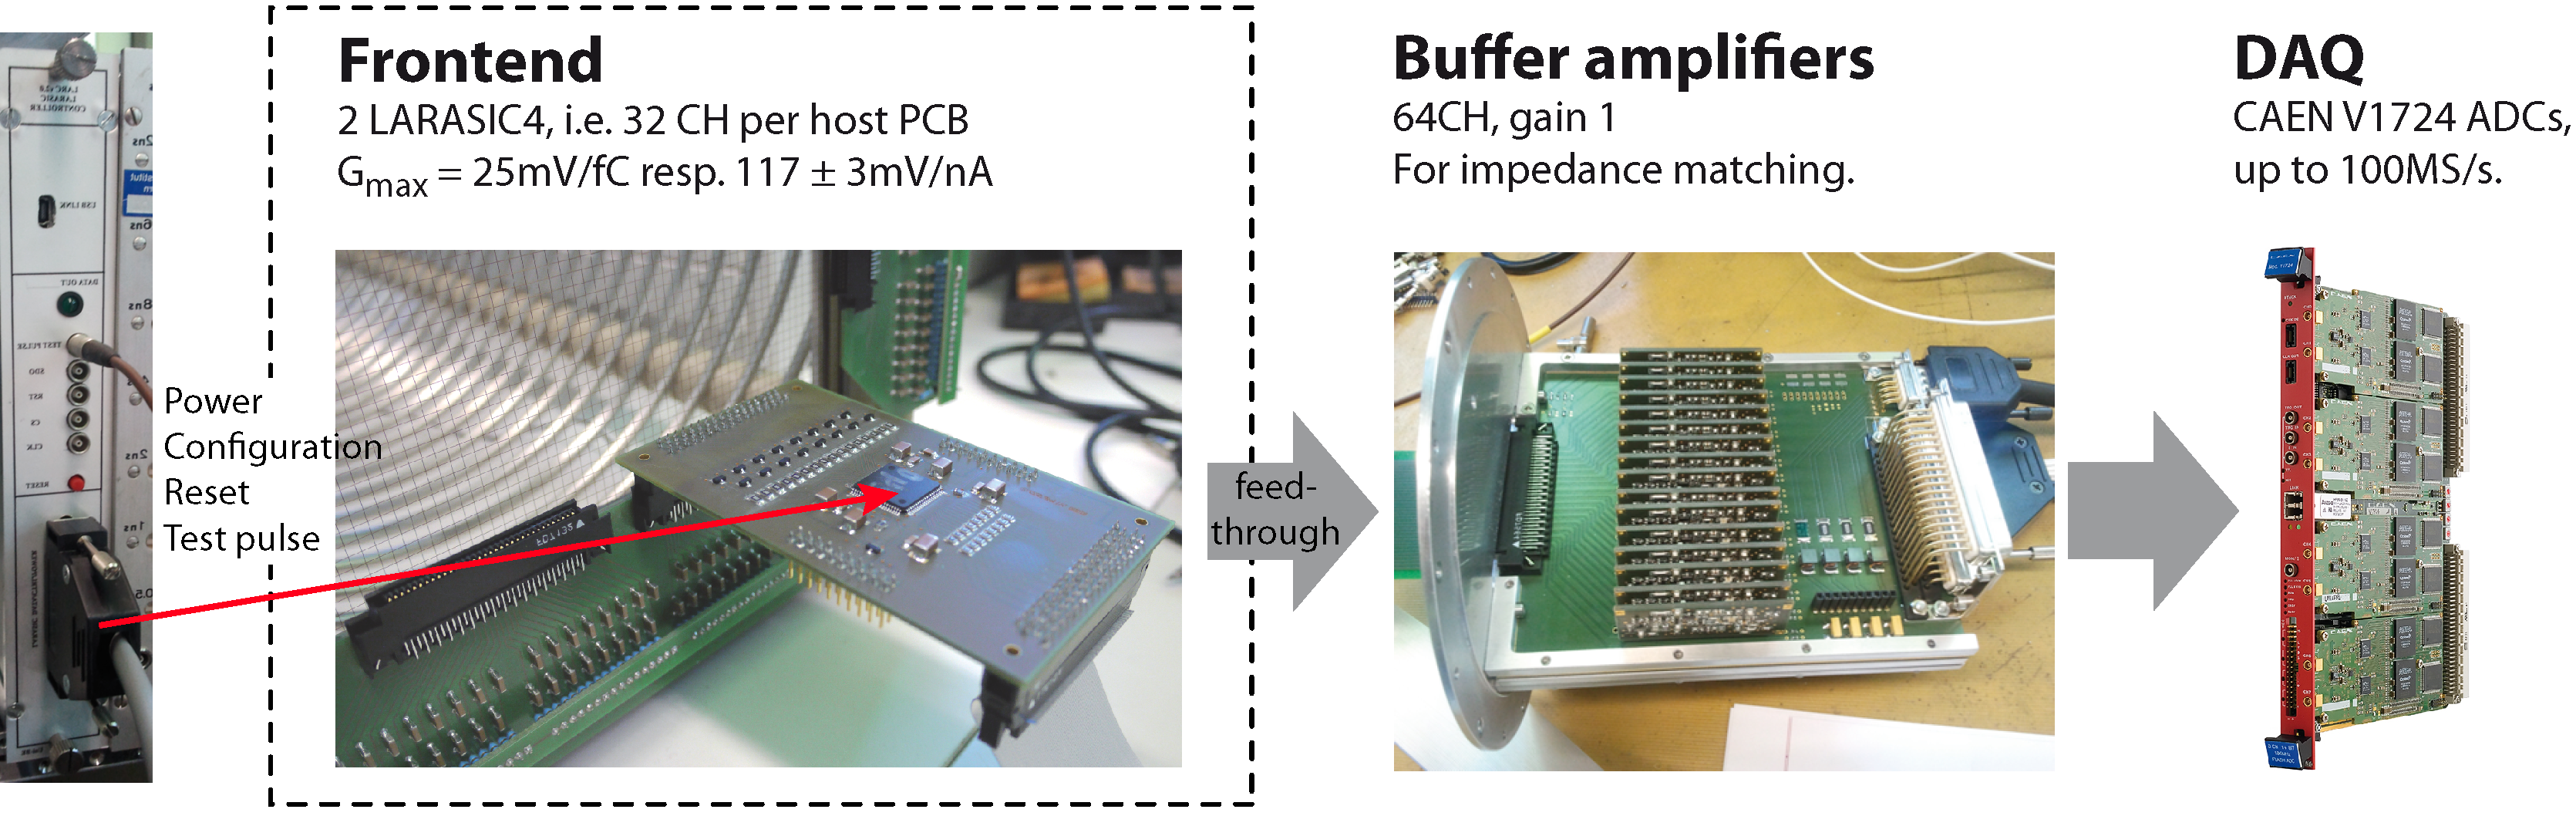
\includegraphics[width=\textwidth]{viper/ReadoutChain_old}
	\caption{Readout chain used for the pixel test. The picture of the LARASIC cryogenic front-end preamplifiers shows them installed in an older wire readout setup.~\cite{AT_larasic}}
	\label{fig:viper_readoutChain_old}
\end{figure}

The cryogenic preamplifiers are mounted to PCBs connected to the back of the pixel readout plane.
Via an inter-integrated circuit (I$^2$C) bus, the LARASICs can be programmed to the different aforementioned configurations.
For this purpose, they are connected to a bespoke NIM module housing an Arduino which generates the I$^2$C signals, a test pulse generator, and multiple low-noise voltage regulators providing power to the LARASICs.
By means of flexible Kapton ribbon cables, the output of the preamplifiers is fed to buffer amplifiers mounted on top of the signal feedthrough.
The latter operate at room temperature, have a unity gain, and match the output impedance of the LARASICs to the \SI{50}{\ohm} input impedance of the downstream digitisers.
From the buffers, the signals are routed via \SI{50}{\ohm} unbalanced coaxial lines to \emph{CAEN V1724}\footnote{\href{http://www.caen.it}{http://www.caen.it}} \SI{14}{bit} digitisers sitting in a VME crate.
For debugging purposes, the output of the buffers can be routed to an oscilloscope via a coaxial T-piece.
Finally, the digital data is read out from the VME crate via a fibre-optic link by a standard PC.
Figure~\ref{fig:viper_readoutChain_old} depicts the entire readout chain.
The complete analogue signal path from the pixel plane to the VME digitisers is single-ended and thus prone to ground loops and all the accompanying noise problems.


\section{Tunings after the first measurement campaign\label{sec:rd-dune-nd_tuning}}

\begin{figure}[htb] %TODO: picture
	\centering
	
\includegraphics[width=\textwidth]{placeholder}
	\caption{Event from the first measurement campaign of the pixel prototype.}
	\label{fig:viper_noisy-event}
\end{figure}

During the first measurement campaign using a pixelated readout, it became apparent that the data is significantly impaired by noise.
As can be seen in Figure~\ref{fig:viper_noisy-event}, the noise amplitude is similar over multiple channels.
This implies a common mode component that cannot originate from inductive pickup.
Instead, the noise is likely generate by self-oscillating parts of the signal path due to ground loops and parasitic impedances.
For the second measurement campaign, different measures were take to mitigate this behaviour.

The first measure was to build a decoupled clean power grid in the lab.
A motor generator (M-G set) separates the special grid mechanically from the building power supply.
Thus, any noise present on the latter is prevented from entering the experimental setup.
Furthermore, this decouples the special grid entirely from the building ground preventing ground loops via the power supply.

A second measure consisted of changing the signal path from the impedance matching buffer amplifiers to the digitisers---i.e. the warm signal path---from single-ended to differential signalling.
For conventional single-ended signalling, the signal is measured as the voltage or current difference between a signal conductor and a ground common to the signal source and the signal sink.
Using a common ground as signal return path can have several undesired effects.
To shield the signal conductor, it is usually enclosed in a ground shield.
If the latter is connected on both sides, a ground loop can result for instance in combination with a shared power supply ground.
Ground loops can pick up noise through induction if the resistance along the loop is high enough.
A second way to couple noise into a single-ended system is by shifting the potential on the common ground away from the reference voltage or current, for instance due to high currents flowing through a lossy ground connection.
Because the signal is always measured against the common ground, it will be distorted.
In differential signalling, the signal is not measured between a signal conductor and ground but instead between two signal conductors.
This works by putting an inverted waveform of the signal on a second conductor.
The signal is recovered by taking the difference between to two signal conductors.
As a result, the signal sink needs not be connected to the same ground as the signal source because the signal is independent of ground.
Ground loops can thus be avoided in the signal path.
Furthermore, the effects of noise pickup on the signal lines is drastically reduced.
Due to the completely symmetric signal path, inductive noie pickup is equal on both signal conductors as opposed to single-ended signals where the signal path is not symmetric.
In the signal sink, the difference between the two symmetric signal conductors is formed and everything that is present on both of them such as the inductively picked up noise cancels out.
In the pixel prototype setup, differential signalling was realised by replacing the buffer amplifiers by single-ended to differential amplifiers and inserting another stage upstream of the digitisers to change the signal back to \SI{50}{\ohm} single-ended, matching the input of the digitisers.
Like this, noise pick up outside the cryostat could be reduced as well as sensitivity to ground loops between the detector and the DAQ rack.

A third source of noise was identified in the layout of the pixel readout plane.
It was found that due to several ground planes and long tracks in the PCB, parasitic capacitances were very high, in particular for pixel channels.
This is problematic because for high enough frequencies---determined by $RC$---, the input is shorted to ground creating a ground loop again.
Through this capacitive coupling to ground, the system can start to oscillate.
One evidence for this is that the noise is equal over multiple channels, so-called common-mode noise.
More specifically, the noise is equal over groups of channels.
Investigating this, it was found that these groups correspond to channels of roughly equal parasitic capacitance.
Also, the noise amplitude is higher on channels with higher capacitance.
To solve this problem, the PCB design was optimised by removing unnecessary ground planes, routing signal tracks outside necessary ground planes and increasing the thickness of the PCB.

\begin{figure}[htb] %TODO: picture
	\centering
	
\includegraphics[width=\textwidth]{placeholder}
	\caption{Event from the second measurement campaign of the pixel prototype after improving the readout chain.}
	\label{fig:viper_good-event}
\end{figure}

As can be seen from Figures~\ref{fig:viper_noisy-event} and~\ref{fig:viper_good-event}, there is a significant decrease in noise after commissioning all of the above improvements to the readout chain.
This can also be seen from Figures~\ref{fig:viper_snr-noisy} and~\ref{fig:viper_snr-good} depicting the signal to noise ratio of the two measurement campaigns.

\begin{figure}[htb] %TODO: picture
	\centering
	
\includegraphics[width=\textwidth]{placeholder}
	\caption{Signal vs noise using the old readout chain.}
	\label{fig:viper_snr-noisy}
\end{figure}

\begin{figure}[htb] %TODO: picture
	\centering
	
\includegraphics[width=\textwidth]{placeholder}
	\caption{Signal vs noise after imrpoving the readout chain.}
	\label{fig:viper_snr-good}
\end{figure}


\section{3D reconstruction\label{sec:rd-dune-nd_reco}}
To characterise the pixel readout, together with the Bern group I will implement a truly 3D reconstruction in the LArSoft framework.
This allows the comparison of the pixel readout performance with contemporary projected wire readouts.
To have a direct comparison, we use 2D projections of the data taken with the pixels, thus eliminating any bias not related to projection.
This enables future experiments to reconstruct data from pixelated readouts.


\section{Simulation\label{sec:rd-dune-nd_simulation}}
Establishing a simulation of the pixelated readout assists its design and implementation in future detectors, which will be especially important for the physics requirements of those detectors.
An important outcome is the influence of the module walls on reconstruction efficiencies.
They can be regarded as missing pixels in the simulation.
My task is to implement the actual pixel readout into existing simulations of future detectors in the beginning of 2017.
